\documentclass[12pt]{standalone}

\usepackage{tikz}

\tikzset{real edge/.style={black,solid,very thick}}
\tikzset{virtual edge/.style={black,dashed,thin}}

\begin{document}
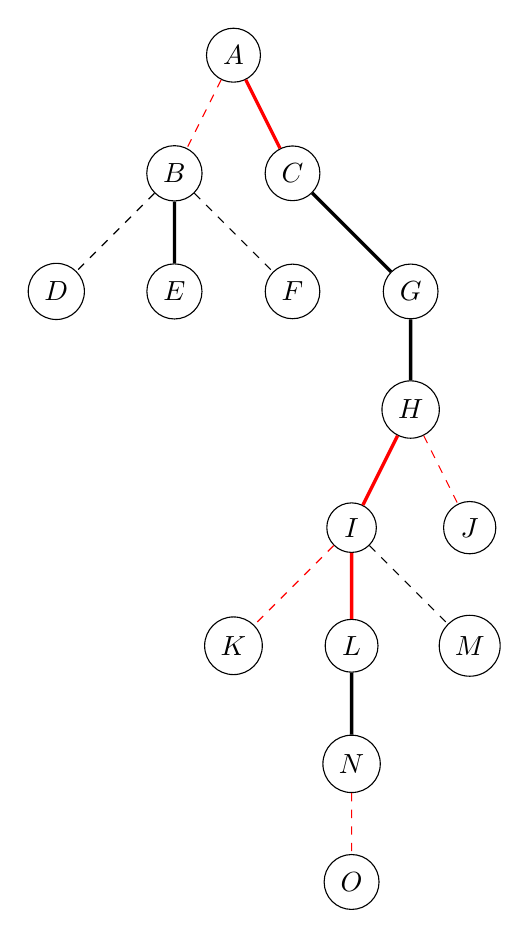
\begin{tikzpicture}

\scoped[every node/.style={black,solid,thin,circle,draw}]
\node {$A$}
    child[virtual edge,red] {node {$B$}
        child[virtual edge] {node {$D$}}
        child[real edge] {node {$E$}}
        child[virtual edge] {node {$F$}}}
    child[real edge,red] {node {$C$}
        child[missing]
        child[missing]
        child[real edge] {node {$G$}
            child[real edge] {node {$H$}
                child[real edge,red] {node {$I$}
                    child[virtual edge,red] {node {$K$}}
                    child[real edge,red] {node {$L$}
                        child[real edge] {node {$N$}
                        child[virtual edge,red] {node {$O$}}}}
                    child[virtual edge] {node {$M$}}}
                child[virtual edge,red] {node {$J$}}}}};

\end{tikzpicture}
\end{document}
